%Edit 0026 ZZZ to report number nnnn 
%Edit  YYMILE to milestone number m.m.m
%Edit exc  ep  Acronyms and Symbols YYTITLE to report title - Words Start with Caps
\documentclass[11pt,twoside,a4paper]{article}
%%======================================================================
%% PACKAGES:
%%
%\usepackage{times}               % Times+Helvetica+Courier fonts
\usepackage{helvet}              % helvetica + cmr
\usepackage{fancyhdr}       % package for headers/footers
\usepackage{amsmath}
\usepackage{amssymb}
\usepackage{graphicx}            % Graphics.
%\usepackage{a4}                  % page layout to fit A4
%\usepackage{lastpage}            % get page no of last page
%\usepackage{ifthen}              % logical branching
\usepackage{hyperref}            %insert hyper-links
\usepackage{latexsym}
\usepackage{longtable} % insert tables that break over pages
\usepackage[acronym]{glossaries} % acronym option makes a separate list for acronyms
% uncomment the following to override auto page total
%\pptotal{20}
%%======================================================================

% ensure sans-serif font used throughout
\renewcommand{\familydefault}{\sfdefault}

\newcommand{\culhamissueno}{1.00}%<==edit
\newcommand{\culhamshorttitle}{CD/EXCALIBUR-FMS/0026}%<==edit
\newcommand{\Sec}[1]{Section~\ref{sec:#1}}
\newcommand{\Fig}[1]{Figure~\ref{fig:#1}}
\newcommand{\Tab}[1]{Table~\ref{tab:#1}}
\newcommand{\Eq}[1]{Equation~(\ref{eq:#1})}
\newcommand{\Eqs}[2]{Equations(\ref{eq:#1}) and~(\ref{eq:#2})}
\newcommand{\Figs}[2]{Figures~\ref{fig:#1}--~\ref{fig:#2}}
%Bold lc for script names, tt for computer code and file-names
%\F{NEPTUNE} always in caps
\newcommand{\F}[1]{\textsc{#1}}
\newcommand{\B}[1]{\textbf{#1}}
\newcommand{\T}[1]{{\tt #1}}
\newcommand{\V}[1]{\mathbf{#1}}
\newcommand{\I}[1]{\textit{#1}}
\newcommand{\nep}{\textsc{NEPTUNE}}
\newcommand{\exc}{\textsc{E}x\textsc{CALIBUR}}
\newcommand{\Papp}{Proxyapp}
\newcommand{\papp}{proxyapp}



%%======================================================================

%% REPORT COVER PAGE Information

\newcommand{\culhamtitle}{\LARGE \exc \ \nep \  Acronyms and Symbols}%<==edit

%%QA BOX information -- change following as needed
\newcommand{\culhamboardname}{Martin O'Brien}%<==edit
\newcommand{\culhamcontactname}{Rob Akers}%<==edit
\newcommand{\culhamauthor}{Wayne Arter}%<==edit
\newcommand{\culhamauthora}{Ed Threlfall}%<==edit
\newcommand{\culhamauthorb}{Joseph Parker}%<==edit
%\newcommand{\culhamcontacttel}{Telephone: 01235 466498}
%\newcommand{\culhamcontactemail}{Email: rob.akers@ukaea.uk}

\newcommand{\culhamdate}{\today}%<=edit
\newcommand{\culhamdatea}{\today}%<=edit
\newcommand{\culhamdateb}{\today}%<=edit

% reproduce Rob's page size

\setlength{\textheight}{220.0mm}
\setlength{\textwidth}{165.0mm}
\setlength{\topmargin}{0.0mm}
\setlength{\oddsidemargin}{0.0mm}
\setlength{\evensidemargin}{\oddsidemargin}
\setlength{\parindent}{0mm}
\addtolength{\parskip}{0.5\baselineskip}
\setlength{\topsep}{0pt}
\setlength{\itemsep}{0pt}

% make glossaries - must be called after \usepackage{hyperref}
\makeglossaries
% glossary entries can be defined in the main body, but it's recommended to
% define them in the preamble
\newglossaryentry{computer}
{
  name=computer,
  description={is a programmable machine that receives input,
               stores and manipulates data, and provides
               output in a useful format}
}

\newglossaryentry{pi}
{
  name={\ensuremath{\pi}},
  description={ratio of circumference of circle to its
               diameter},
  sort=pi
}




\newacronym{ANL}{ANL}{Argonne National Laboratory}
\newacronym{ANN}{ANN}{Artificial neural network}
\newacronym[longplural={analyses of variance},shortplural={ANOVAE}]{ANOVA}{ANOVA}{analysis of variance}
\newacronym{API}{API}{Application Programming Interface}
\newacronym{ASQ}{ASQ}{Adaptive sparse quadrature}
\newacronym{ATS}{ATS}{Advanced Terrestrial Simulator, previously Arctic Terrestrial Simulator}
\newacronym[longplural={Frames per Second}]{fpsLabel}{FPS}{Frame per Second}


%%======================================================================
\begin{document}

%Titlepage comes out wrong size, but should look right apart from
% picture which cannot be wider than c.150mm.
% To produce conforming report rp1pub.pdf
% remove title page by commenting out lines ending in %<==omit, then
% sed -e '/<==omit$/s/^/%/' < rp1.tex > rp1omit.tex
% pdflatex rp1omit;bibtex rp1omit; pdflatex rp1omit
% pdfunite cover.pdf rp1omit.pdf rp1pub.pdf 
\begin{titlepage}%<==omit
\vspace*{-30mm}%<==omit

\includegraphics[width=2.5cm]{../corpics/cofaplus} \\[2.0\baselineskip]%<==omit
{\LARGE {\textbf{\textsf{ExCALIBUR}}}}\\[2.0\baselineskip]%<==omit
{\LARGE \culhamtitle } \\[2.0\baselineskip]%<==omit
{\textbf{\textsf{Abstract}}}\\%<==omit
The report describes acronyms, conventions and symbols for \exc \ project \nep. %<==omit
Report on the status of programming models and code generators for the
various node architectures focused on performance, usability, maintainability
and  availability.  
%<==omit
%<==omit
\vfill%<==omit
\centerline{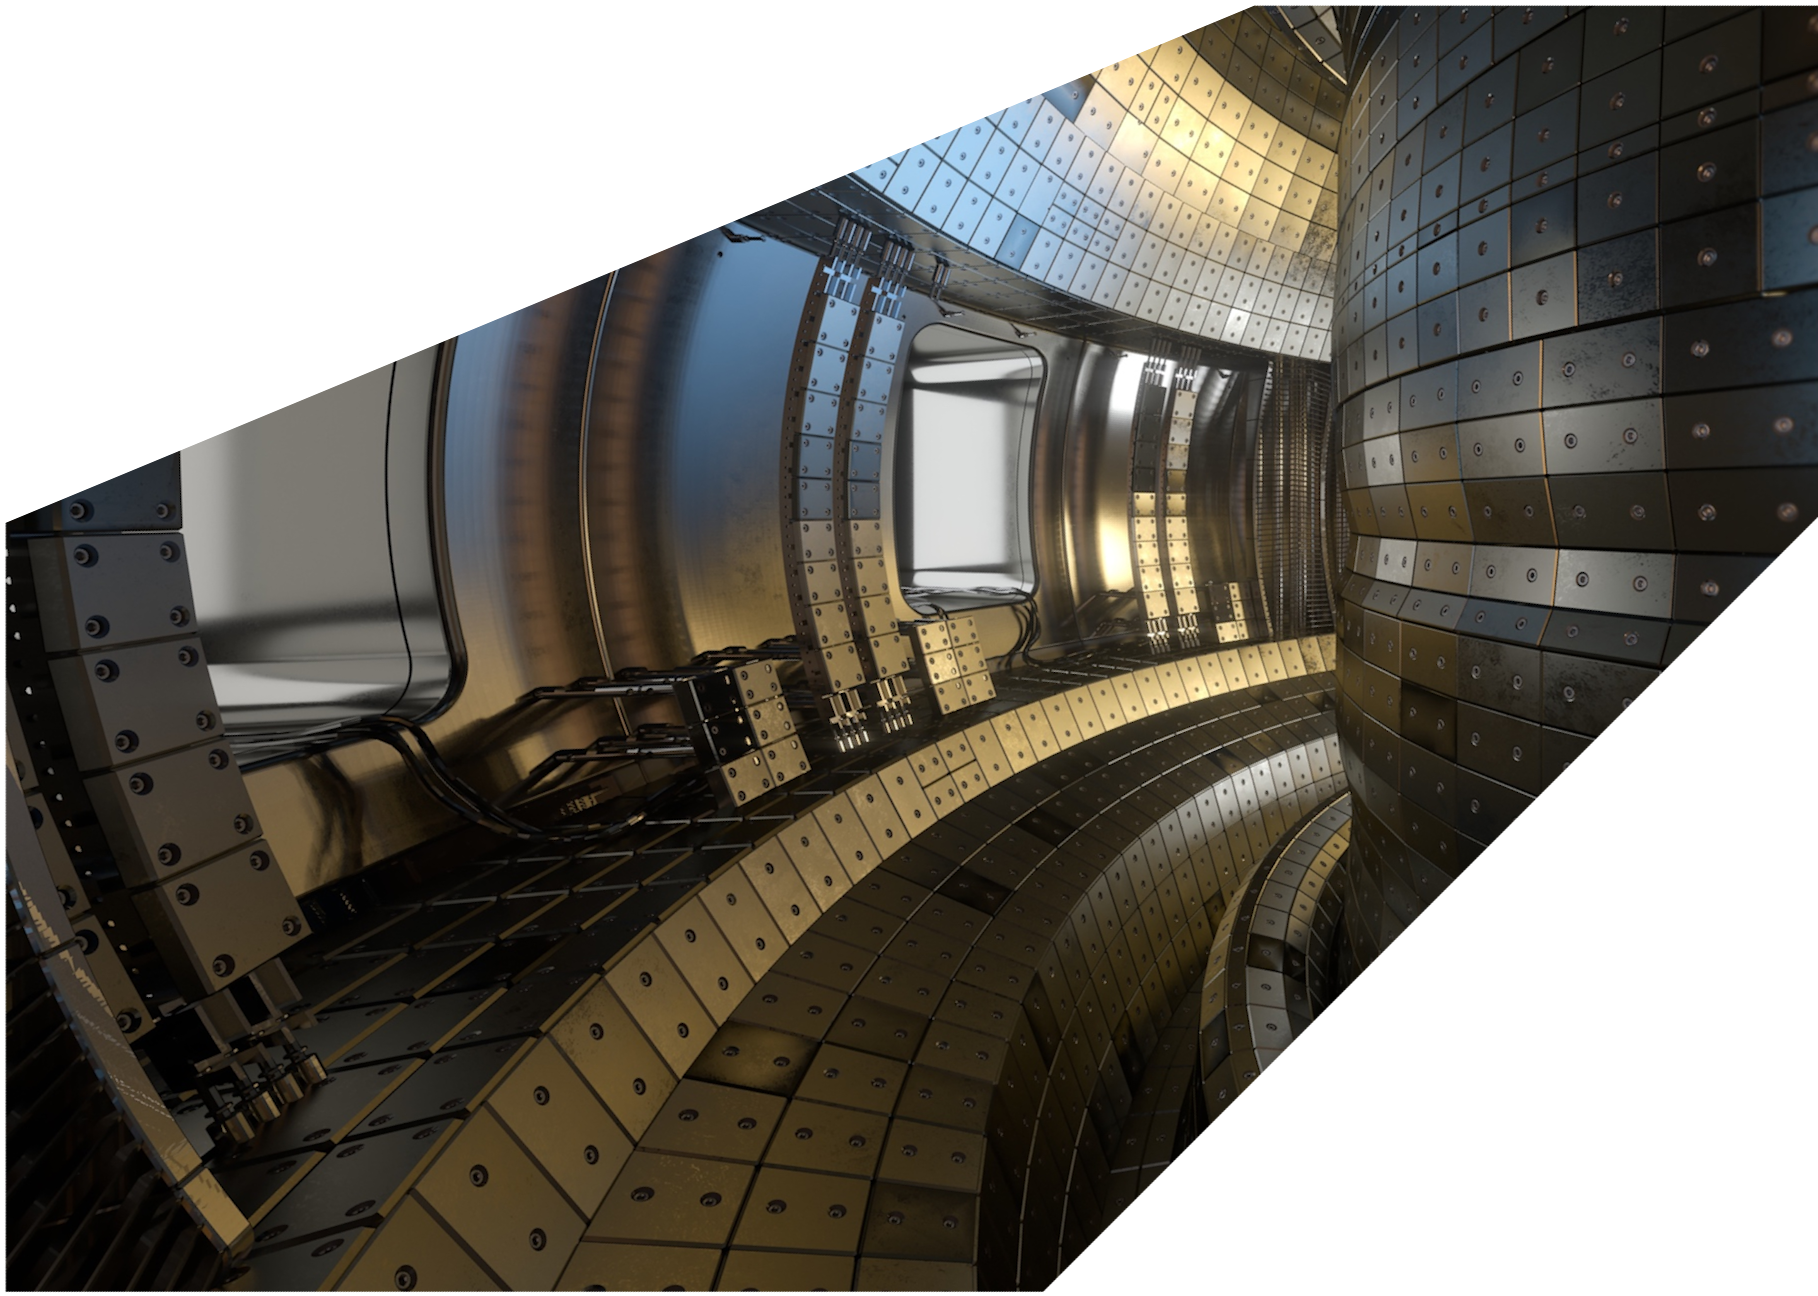
\includegraphics[width=0.9\textwidth]{../corpics/tokintcrop}}%<==omit
\end{titlepage}%<==omit

\hspace{-30mm}\begin{table}[h]
\sffamily
\begin{center}
\textbf{\textsf{UKAEA REFERENCE AND APPROVAL SHEET}}
\begin{tabular}{||p{5.7cm}|p{4.7cm}|p{5.0cm}||}
\hline
\hline
& Client Reference: &  \\
\hline
& UKAEA Reference: & \culhamshorttitle \\
& & \\
\hline
& Issue: & \culhamissueno \\
\hline
& Date: & \culhamdateb \\
\hline
\multicolumn{3}{||l||}{} \\
\multicolumn{3}{||l||}{Project Name: ExCALIBUR Fusion Modelling System} \\
\multicolumn{3}{||l||}{} \\
\hline
\end{tabular}
\begin{tabular}{||p{3.3cm}|p{4.6cm}|p{3.5cm}|p{3.6cm}||}
\hline
& Name and Department & Signature & Date \\
\hline
Prepared By: & \culhamauthora & N/A & \culhamdate \\
& \culhamauthor & N/A & \culhamdate \\
%& \culhamauthorb  & N/A & \culhamdate \\
%& \culhamauthorc  & N/A & \culhamdate \\
& & & \\
& BD & & \\
\hline
Reviewed By: & \culhamcontactname & 
\includegraphics[width=3.0cm]{../corpics/blanksign}& \culhamdatea \\
& & & \\
& Advanced Computing Dept. Manager & & \\
\hline
%Approved By: & \culhamboardname  & \includegraphics[width=3.0cm]{../corpics/mobsign} & \culhamdateb \\
%& & & \\
%& MSSC & &\\
%\hline
\hline
\end{tabular}
\end{center}
\end{table}


\clearpage
\section{Introduction}\label{sec:intro}
This report collates technical material used to inform the preparation of the call for 
procurement of support for Uncertainty Quantification~(UQ).
The work performed primarily consisted of collating material produced
internally~\cite{y2re241,y2re242,y2re251,y2re313}
and by external grantees at UCL~\cite{2047352_1-TN-01,2047352_2-TN-01}, plus
hands-on exploration of sampling techniques, the construction of surrogates and the study
of dimensionally reduced models.
The production of this call reflects the importance attributed to UQ in project \nep, so that 
the software produced should be capable of producing `actionable' results, that could form a significant
input to multi-million pound procurements.

It seems worthwhile to start by recapitulating the project
\nep \ requirements for UQ, insofar as they are currently understood. In particular, to
note a clear distinction between the experiments that \nep \ code needs to model, and the
outputs of the simulations themselves.  Relevant experiments are almost entirely medium-sized
and large tokamaks, where it seems that even the edge plasma has a temperature of
around~$10$\,eV~($10^5$\,K). The presence of magnetic fields of order $1-10$\,T, and
electric fields of around $10^4$\,Vm$^{-1}$ implies a hostile environment, subject further
to large electromagnetic transients not just at start-up and ramp-down of a discharge, but also caused by
plasma instabilities such as ELMs and sawteeth.  Most diagnostics struggle to achieve absolute
accuracies of $10$\,\%, although they usually detect the direction of smaller changes reliably.
Many are ``one-of-a-kind" so require careful interpretation, and all signals may have been subject to
filtering both at low and high frequencies, to remove  `spikes' and `drift'.
In comparison, signals from simulation are very `clean', but the simulation may lack
crucial realism, in that either important physical processes are not treated or 
if included, that the spatio-temporal discretisation may not be sufficiently fine to
represent them accurately.

%The Model  expt. - noisy, large unc. toks
%simulation - clean, level of detail controllable by mesh refinement, more detailed physics

Turning to the expected usage of the \nep \ software, this covers  both physics and engineering.
Both physicist and engineers are potentially interested in everything computed by the software, which is of course
likely to be an overwhelming amount of detail. A physicist is more likely to begin by
formulating simpler models and use the software to determine their appropriateness and accuracy,
an engineer probably more likely to use the output of simulation as a basis for producing simplified models.
An experimental physicist may be satisfied with qualitative accuracy, provided it is obtained
rapidly enough to help formulate the next experimental `shot' (eg.\ by indicating that more
or less gas input would be helpful), whereas a more theoretical
%counterpart may want a model useful for extrapolation to reactor parameters. An engineer
counterpart may want to quantify the difference between model predictions and experiment 
sufficiently well to help produce a more refined model. An engineer
seeking to design a reactor may be interested only in a relatively small number of
quantities of interest~(QoI) but which need to be determined more precisely, 
such as local maxima in time-averaged heat flux, whereas
other engineers may see edge code as forming a part of a digital twin, to be used to help control
operation of an actual tokamak device where accurate time-dependent modelling will also be critical.
%Users physicist -  formulate simpler models useful for extrapolation of geometry and parameter changes
%potentially interested in everything as extrapolation
%experimental physicist, qual accuracy OK for fuelling
%engineering design - few QoI, static
%digital twin (as part) - for operation and control, quant accuracy, time dep.
It is notable that most of the preceding requirements involve extrapolation,
from model to new features of an existing experiment or, in the design case, to more
extreme values of geometrical size, magnetic field etc. representing a fusion reactor
relative to existing experiments such as JET.
%Requirements - interpolation, to obtain sufficient data to perform to a given accuracy
%extrapolate - "to expt" and to new parameters

For the above it is therefore as Smith~\cite{smithUQ} describes (see also the \nep \
report~\cite[\S\,1]{y2re313}), important that UQ involves more than just clever sampling
to identify parameter sensitivities, and the standard definitions of ways of quantifying
these such as Sobol indices~\cite{y2re241}. In particular,
the production of surrogate models is within scope of UQ.
%sampling imp. for identifying important parameters
It is worth saying that in one sense even the most complex partial differential equation~(PDE) models of plasma are 
simply surrogates for experimental `reality'. The most detailed and least controversial
model of tokamak plasma consists in treating it as of order~$10^{20}$ or more particles evolving
under the influence of external and self-generated electromagnetic fields, but
this is of course not tractable even at the Exascale~\cite{Wa95a}, without very selective
sampling of the particles. Currently, particle models are seen as at best struggling to capture
edge plasma behaviour, with no certain likelihood of significant improvement, and 
in any event there is a separate calls that could cover research into particle sampling. The PDE models
attempt to capture the key physics of the plasma particles, viz.\ their appearance, motion,
interactions with other particles and eventual loss, as terms representing respectively
source, advection, diffusion and sinks in continuum models. Unfortunately, long mean free
paths~(\emph{mfp}s) mean that at least in some regions it is necessary explicitly to represent
phase-velocity dependence of plasma density, and the resulting basic 6-D dependence of 
fields (5-D if gyro-averaged models are used) stretches current and foreseen computing
facilities. In any event, above applications eg.\ preliminary design studies and operational control,
require models capable of evaluation within seconds or less, ie.\  surrogates for the
PDEs, expected to have lower spatial dimensionality (2-D or 1-D) or even as systems of 
ordinary differential equations~(ODEs).
%Surrogate. PDE solution as surrogate for expt/reality, advection, diffusion, sinks and sources.

Unfortunately for application to \nep, most surrogates have been designed for use as
interpolants. Nonetheless, interpolation is likely to be important at least within the software,
eg.\ to connect different models, and the book by de~Boor~\cite{deboor} has interesting
material relating to the use of splines in this context. In particular, de~Boor lists
theorems relating to the optimality of spline polynomial interpolation, so that there might be
wonder that any other form of interpolation is required. In fact, spline optimality is found only in 
the energy or least-squares norm, so there is anyway the possibility of fitting the data
with polynomial functions that have under- and over-shooting oscillations between sample
points (called nodes in spline jargon). Moreover, de~Boor illustrates the potential for dramatic failings
using what he refers to as the Titanium heat data set~\cite[Fig.\ XIII.1]{deboor}. The data is
a set of some~$50$ apparently regularly spaced samples of a function which is practically
flat except for one distinct `hump', rising to four times the value of the `plateau' over
c.\ $15$\,\% of the range. Since the interpolation is by a piecewise  ($5^{th}$ order polynomial)
the undershoot by greater than the maximum `hump' value is in many respects more impressive than
that exhibited in Boyd's book~\cite[Fig.\ 4.3]{boyd} as part of his demonstration of the Runge
phenomenon, ie.\ that polynomial interpolation at evenly spaced points may diverge. In both books,
the problem is identified as due to poor choice of sample points. de Boor~\cite[Fig.\ XIV.5]{deboor}
shows improved fitting if the number of samples in the plateau region of the \emph{Ti} heat data is reduced,
whereas Boyd points out that optimal $N^{th}$~order polynomial interpolation is achieved using
sample points that are the roots of the Chebychev
polynomial of degree~$(N+1)$, that cluster as close together as~$1/N^2$ near the end-points
of the sample region. In any event, for many interpolation purposes, it seems that polynomial spline
fitting with an order of three or so, is adequate \emph{provided} the nodes are chosen suitably. The cost
scales as the operation count  of a banded-diagonal matrix solver, so~$\mathcal{O}(N)$ where $N$~is the
number of points to be interpolated per dimension.
There are however strong proponents for the use of rational polynomial interpolation~\cite{stoerbulirsch}
and in particular radial basis function~\cite{fornbergflyer}. Wavelet bases~\cite{Fa15Wave} also
have their adherents, and special conditions such as periodicity or infinite domain mean that
respectively Fourier series and the Hermite basis are to be preferred. The Hermite basis is
employed in the Polynomial Chaos Expansion~(PCE), which is advocated by P.\ Coveney~et~al, see
the \nep\ report~\cite{2047352_1-TN-01}. % and special bases will not be discussed further

Accurate spline fitting requires a sufficient amount of data to enable best location of the
nodes, which, since they generally aim to use as few nodes as possible, is commonly unavailable
in the output of
highly expensive numerical calculations. This lack of data means also that interpolation using
Neural Networks~(NNs)  is mostly unsuitable, and motivates the use of Gaussian Processes~(GPs)
for interpolation despite their expense, that~$\mathcal{O}(N^3)$ of inverting a full matrix~\cite{y2re242}.
They come with the benefit of accompanying error bounds, and seem to be relatively stable when
used for extrapolation~\cite{Ch20priv}. They may be very effective in combination with a 
special basis produced by Principal Component Analysis~(PCA), \emph{aka} Proper Orthogonal Decomposition
or POD, see the \nep\ report~\cite{2047352_2-TN-01}. Moreover, S.~Guillas~\cite{Li17Dime} describes
a number of techniques which outperform PCA, in particular favouring a reproducing kernel
approach to estimating derivatives needed to optimise the basis. This is coupled with
a sequential approach to selecting sample points.
Indeed, choosing sample points appropriately is still a major issue for GPs, which P.~Challenor (private
communication) has explored extensively and favours `Leave One Out'~(LOO).

% as interpolant (1) polynomial spline, GP, NN.
%limitations of spline, GP and NN in table/appendix.
%De Boor for spline, Ti heat data XIII.1 - Gibbs like phena - but XIV.5 shows OK if get nodes
%in right place
Nonetheless, given the general need for extrapolation, it is desirable to incorporate as much
physical knowledge as possible into the surrogate model. The hopes are that the parameters
of the surrogate are either invariant under the extrapolation, or that they have well-determined
scaling properties, and that all important physical processes have been identified.
The parameters of the surrogate may then be fitted using existing data from
experiment and/or simulation as described above.
The surrogate may need to be space and/or time dependent as required by the
user and application. Of course, such surrogates can be very useful for interpolation also.
Worthy of particular mention is Model Order Reduction~\cite{y2re251}, which for linear and some nonlinear
problems, offers reliable estimates of error in interpolating Quantities of Interest~(QoI),
hence likely to be particularly useful for the design engineer.

The body of the current document consists of hands-on exploration of sampling techniques
in \Sec{bout}, the construction of surrogates by Gaussian Processes in \Sec{nektar} and
of surrogates consisting of dimensionally reduced models in \Sec{dimred}.
The implications for the call are summarised in \Sec{summ}.

\clearpage
\section{Acronyms}\label{sec:acro}
Acronyms used in t31 work to go here from file t31acro.txt.

One of my favourite statistical techniques is \gls{ANOVA}.
The full name and acronym are printed on first usage, but thereafter the same command prints ``\gls{ANOVA}''.
\glsreset{ANOVA}
Calling \verb+\glsreset{ANOVA}+ means the full name is printed next time we write \gls{ANOVA}.
\glsreset{ANOVA}
\Gls{ANOVA} is capitalized by using \verb+\Gls{ANOVA}+, while the plural is provided by \verb+\glspl{ANOVA}+, giving \glspl{ANOVA} or, after resetting,
\glsreset{ANOVA}
\glspl{ANOVA}.
The (possibly incorrect) ``analyses of variance'' and (definitely incorrect) ``ANOVAE'' plurals are produced by the `longplural' and `shortplural' optional arguments to \verb+\newacronym+.
Without these, the defaults would be ``analysis of variances'' and ``ANOVAs''.

By default, only acronyms that are referenced are included in the glossary.
This makes it difficult for the glossary to be a separate document from the reports (and it certainly breaks the page number cross-referencing).
One work-around for this would be to use the command \verb+\glsaddall+ to include all terms in the glossary file, and then turn off the page numbers by including the argument \verb+[nonumberlist]+ in the \verb+usepackage+ command.

\glsaddall



\printglossaries

%\begin{longtable}[h]
%\begin{center}
\begin{longtable}{|p{4.0cm}|p{12.0cm}|}
\hline
ACM & \\
ADC & \\
AMR & \\
AMReX & \\
AND & \\
ANL & Argonne National Laboratory \\
ANN & Artificial neural network \\
ANOVA & Analysis of Variance \\
API & Application Programming Interface \\
ASQ & Adaptive sparse quadrature \\
ATS & Advanced Terrestrial Simulator, previously Arctic Terrestrial Simulator \\
AUXVAL & \\
BD & \\
BG/L & \\
% BOUT++ & proper noun not acronym
BOX & \\
BP & \\
CabanaMD & \\
ECP-copa & \\
CCFE & Culham Centre for Fusion Energy \\
CD & \\
CEA  & \\
CESM & \\
CI & \\
COGENT & \\
COMPAT & \\
COSMO & \\
COSSAN & \\
CPP & \\
CPU & Central Processing Unit \\
CRC & \\
CS & Compressed sensing \\
CSE & \\
CSMP & \\
CTO & \\
CUDA & Compute Unified Device Architecture \\
CWIPI & \\
DAG & Direct Acyclic Graph \\
DAKOTA & \\
DDA & \\
DFT & Discrete Fourier Transform \\
DOE & Department of Energy \\
DOI & Digital Object Identifier \\
DSL & Domain-Specific Language \\
ECP & \\
EIRENE & \\
ESI & \\
ESMF & \\
ETS & \\
EU & European Union \\
FACETS & \\
FCI & Flux-Coordinate Independent (methods) \\
% FELTOR proper noun
FEM & Finite Element Method \\
FEniCS & \\
FFT & Fast Fourier Transform \\
FFTW & Fastest Fourier Transform in the West (library) \\
FLASH & \\
% FORTRAN
% FORTRAN~77
GA & General Atomics \\
GBD & \\
GBS & \\
GDB & \\
% GENE proper noun?
GMRES & Generalized Minimal Residual method \\
GNU & GNU's Not Unix! \\
gPC & Generalised polynomial chaos \\
GPU & Graphics Processing Unit \\
% GRILLIX proper noun?
GSA & Global sensitivity analysis \\
GUI & Graphical User Interface \\
HDF5 & Hierarchical Data Format (version 5) \\
HLA & \\
HPC & High Performance Computing \\
HVAR & \\
% IBM & International Business Machines Corp., but really known as IBM \\
ICON & \\
IEEE & \\
IMAS & \\
IMEX & Implicit-Explicit Methods \\
IO & \\
% ITER *not* International Thermonuclear Experimental Reactor
ITG & Ion Temperature Gradient \\
ITM & Ion Tearing Mode \\
ITPA & \\
JET & Joint European Torus \\
JOREK & \\
LAMMPS & \\
LANL & Los Alamos National Laboratory \\
LASH & \\
LASSO & Least Absolute Shrinkage and Selection Operator \\
LGPL & GNU Lesser General Public License \\
LHSamp & \\
LLNL & Lawrence Livermore National Laboratory \\
MAP & Maximium A Posteriori \\
MC & Monte Carlo (methods) \\
MCMC & \\
MCT & \\
MESAGE & \\
MFMA & \\
MFMC & Multi-fidelity Monte Carlo \\
MHD & Magnetohydrodynamics \\
MIMC & \\
MIT & Massachusetts Institute of Technology \\
ML & Machine Learning \\
MLMC & Multi-level Monte Carlo \\
MLMF & \\
MMF & \\
MOOSE & \\
MOR & \\
MPI & Message Passing Interface \\
MSSC & \\
MUMPS & \\
MUSCLE~3 & \\
% NAG trades a NAG
NEMO & \\
NEPTUNE & \\
NUCODE & \\
OASIS & \\
OASIS4 & \\
OLYMPUS & \\
OMFIT & \\
% OpenMP & Open Multi-Processing, but not really an acronym
OU & Oxford University \\
OUU & Optimisation under uncertainty \\
OUUWA & \\
PASTIX & \\
PC & Polynomial chaos \\
PCE & Polynomial chaos expansion \\
PDE & Partial Differential Equation \\ 
% PETSc & Portable, Extensible Toolkit for Scientific Computation, but again, really it's PETSc
PFC & \\
PGD & \\
PICPIF & \\
POOMA & \\
PP20 & \\
PRESET & \\
QA & \\
QCG  & \\
QMC & Quasi-Monte-Carlo \\
QoI & Quantity of interest \\
RKF23 & \\
ROM & Reduced-order model \\
RNG & \\
SAMRAI & \\
% SD1D name of code
SIAM & Society for Industrial and Applied Mathematics \\
% SLEPc & Scalable Library for Eigenvalue Problem Computations, but really a name
SLSQT & Sequential Least-Squares' Thresholding \\
SMARDDA & \\
SMART & \\
SMITER & \\
SMwiki & \\
SNOWPAC & Stochastic Nonlinear Optimisation with Path-Augmented Constraints (software package) \\
SOL & Scrape-Off Layer \\
SOLEDGE & \\
SOLPS & \\
SRS & \\
STARWALL & \\
STIXGeneral & \\
% STORM
STRUMPACK & \\
% SUNDIALS
SVD & Singular value decomposition \\
SVM & \\
TAE & \\
TM & \\
TOKAM & \\
TOKAM3X & \\
TOMS & \\
TRIMEG & \\
TUM & \\
UK & United Kingdom \\
UKAEA & United Kingdom Atomic Energy Authority \\
UKRI & United Kingdom Research and Innovation \\
UQ & Uncertainty quantification \\
US & \\
USA & \\
UTF-8 & \\
VDE & \\
VECMAtk & \\
VORPAL & \\
XGC1 & \\
XML & \\
XMSF & \\ \hline
\end{longtable}
%\end{center}
%\end{table}

\newglossaryentry{computer}
{
  name=computer,
  description={is a programmable machine that receives input,
               stores and manipulates data, and provides
               output in a useful format}
}

\newglossaryentry{pi}
{
  name={\ensuremath{\pi}},
  description={ratio of circumference of circle to its
               diameter},
  sort=pi
}



\Gls{pi}
\Gls{fpsLabel}

\begin{table}[h]
\textbf{\textsf{TABLE OF SYMBOLS}
Scan of Brunton and Kutz acronyms table converted to text
}
\begin{center}
\begin{tabular}{|p{4.0cm}|p{12.0cm}|}
\hline
\textbf{\textsf{Acronym}}
& \textbf{\textsf{Description}} \\
\hline
ADM  & Alternating directions method \\
AIC  & Akaike information criterion \\
ALM  & Augmented Lagrange multiplier \\
ANN  & Artificial neural network \\
ARMA  & Autoregressive moving averaoe \\
ARMAX  & Autoregressive moving average with exogenous input \\
BIC  & Bayesian information criterion \\
BIM  & Empirical interpolation method \\
BPOD  & Balanced proper orthogonal decomposition \\
CCA  & Canonical correlation analysis \\
CFD  & Computational fluid dynamics \\
CNN  & Convolutional neural network \\
CoSaMP  & Compressive sampling matching pursuit \\
CWT  & Continuous wavelet transform \\
DCT  & Discrete cosine transform \\
DEIM  & Discrete empirical interpolation method \\
DFT  & Discrete Fourier fransform \\
DiMDc  & Dynamic mode decomposition with control \\
DL  & Deep learning \\
DMD  & Dynamic mode decomposition \\
DMDc  & Dynamic mode decomposition with control \\
DNS  & Direct numerical simulation \\
DWT  & Discrete wavelet transform \\
ECOG  & Electrocorticography \\
eDMD  & Extended DMD \\
EM  & Expectation maximization \\
EOF  & Empirical orthogonal functions \\
ERA  & Eigensystem realization algorithm \\
ESC  & Extremum-seeking control \\
FFT  & Fast Fourier transform \\
GMM  & Gaussian mixture model \\
HAVOK  & Hankel alternative view of Koopman \\
ICA  & Independent component analysis \\
JL  & JohnsonLindensfrauss \\
KL  & KullbackLeib1er \\
KLT  & Karhunen-Loeve transform \\
LAD  & Least absolute deviations \\
LASSO  & Least absolute shrinkage and selection operator \\
LDA  & Linear discriminant analysis \\
LQE  & Linear quadratic estimator \\
LQG  & Linear quadratic Gaussian controller \\
LQR  & Linear quadratic regulator \\
LTI  & Linear time invariant system \\
MIMO  & Multiple input, multiple output \\
MLC  & Machine learning control \\
Most  & Common Acronyms \\
MPE  & Missing point estimation \\
mrDMD  & Multi-resolution dynamic mode decomposition \\
NARMAX  & Nonlinear autoregressive model with exogenous inputs \\
NLS  & Nonlinear Schrdinger equation \\
ODE  & Ordinary differential equation \\
OKID  & Observer Kalman filter identification \\
PBH  & PopovBelevitchHautus test \\
PCA  & Principal components analysis \\
PCP  & Principal component pursuit \\
PDE  & Partial differential equation \\
PDE-FIND  & Partial differential equation functional identification of nonlinear dynamics \\
PDF  & Probability distribution function \\
PID  & Proportional-integral-derivative control \\
PIV  & Particle image vetocimetry \\
POD  & Proper orthogonal decomposition \\
RIP  & Restricted isometry property \\
RKHS  & Reproducing kernel Hilbert space \\
RNN  & Recurrent neural network \\
ROM  & Reduced order model \\
RPCA  & Robust principal components analysis \\
rSVD  & Randomized SVD \\
SGD  & Stochastic gradient descent \\
SINDy  & Sparse identification of nonlinear dynamics \\
SISO  & Single input, single output \\
SRC  & Sparse representation for classification \\
SSA  & Singular spectrum analysis \\
STFT  & Short time Fourier transform \\
STLS  & Sequential thresholded least-squares \\
SVD  & Singular value decomposition \\
SVM  & Support vector machine \\
TICA  & Time-lagged independent component analysis \\
VAC  & Variational approach of conformation dynamics \\
\hline
\end{tabular}
\end{center}
\end{table}


\Gls{computer}

\clearpage
\section{Conventions}\label{sec:conv}
\input{conv}
\clearpage
\section{Symbols}\label{sec:symbol}
Symbols Karniadakis and Sherwin to enter in from ksnotn.txt

Symbols used in stage2.tex of t31

\begin{table}[h]
\textbf{\textsf{TABLE OF SYMBOLS}}
\begin{center}
\begin{tabular}{|p{4.0cm}|p{12.0cm}|}
\hline
\textbf{\textsf{Symbol}}
& \textbf{\textsf{Description}} \\
\hline
$[a,b]$ & arbitrary finite interval \\
$d$ & number of dimensions over which the integral is performed \\
$f_0$ & constant in the expansion of $f\left(x_1,\ldots,x_d\right)$ \\
$f\left(x_1,\ldots,x_d\right)$ & joint probability distribution \\
$f_i(x_i)$ & coefficient in the expansion of $f\left(x_1,\ldots,x_d\right)$ \\
$f_{ij}(x_i,x_j)$ & coefficient in the expansion of $f\left(x_1,\ldots,x_d\right)$ \\
$p(x)$ & probability distributions  \\
$r$ & order of higher order term \\
$x_i$ & generic parameter or variable \\ 
${\bf x}=\left(x_1,x_2,\dots,x_d\right)$ & is a $d$-dimensional vector \\
$P(x)$ & Cumulant probability distribution \\
$\parallel  Q \parallel_E $ &the `energy' norm \\
$S_i$ & Sobol sensitivity index, gives a normalised measure of the sensitivity of the distribution of $f$ to the parameter~$x_i$ \\
$S_{ij}$ & Sobol sensitivity index, gives a normalised measure of the sensitivity of the distribution of $f$ to the parameters~$x_i$ and $x_j$ \\
$\mathrm{Var}(f)$ & variance of the distribution of $f$ computed by integrating over all variables~$x_i$ \\
$V_i$ & variance of the distribution of $f$ as the parameter~$x_i$ varies \\
$V_{ij}$ & variance of the distribution of $f$ as the parameters~$x_i$ and $x_j$ vary \\
$\mathbb{E}$ & expectation \\
$\mathbb{E}_{x_{k\neq i}}$ & expectation computed by integrating over all the $x_k$ except for~$x_i$ \\
$\mathbb{E}_{k\neq i, l\neq j}$ & expectation computed by integrating over all the $x_k$ except for~$x_i$ and  $x_j$ \\
$\xi_i$ & randon number within the unit interval~$[0,1]$ \\
\hline
\end{tabular}
\end{center}
\end{table}


\clearpage
\section*{Acknowledgement}\label{sec:ackn}
\emph{The support of the UK Meteorological Office and Strategic Priorities Fund is acknowledged.}


%\section*{References}
\bibliographystyle{unsrt}
\bibliography{../bib/new,../bib/waynes,../bib/misc,../bib/warv,../bib/neuts,../bib/reac,../bib/exc,../bib/active,../bib/dg1srt}

\end{document}
